\documentclass{beamer} 
\usepackage{amsmath,amsthm}
\usepackage{mathrsfs}
\usepackage{amssymb}
\usepackage[english]{babel}
\usepackage{latexsym}
\usepackage{amsfonts}
\usepackage{graphicx}
\usepackage{float}
\usepackage{graphics}
\usepackage{epsfig}
\usepackage{url}
\usepackage{soul}
\usepackage{listings}
\usepackage{bm}

% \usepackage{minted}


\usetheme{WVU}
\usecolortheme{WVU}
\usepackage{multirow}

\mode<presentation> 

\title[VE401 SU2022 Midterm Big RC]{VE401 SU2022 Midterm Big RC}

\author[ Shuyu Wu ]{ Shuyu Wu }
\institute[UM-SJTU JI]{UM-SJTU Joint Institute \vspace{.2cm} \\ 
\includegraphics[scale=0.3]{umji_logo.png}\\wushuyu2002@sjtu.edu.cn}
\date[June 2022]{\today}

\begin{document}
\begin{frame} 

\titlepage 

\end{frame} 
\section{Multivariate Random Variables} 
\begin{frame}
       \frametitle{Outline}
       \tableofcontents[currentsection]
\end{frame}

\begin{frame}
    \frametitle{Discrete Multivariate Random Variables}
    We study discrete random variable and continuous random variable.
    \textbf{discrete random variable}: A map from sample space $S$ to a countable subset of $R^n, \Omega$. i.e., 
    \[\bm{X}: S\rightarrow \Omega\subset R^n\]
    together with a probability
    $\Omega\rightarrow R$ that satisfy
    \begin{enumerate}
        \item $f_X(x)\geq 0 \text{ for }  \forall x=(x_1,x_2,\dots , x_n)\in \Omega$
        \item $\sum\limits_{x\in\Omega}f_X(x)=1 $
    \end{enumerate}
    The function $f_X(x)$ is called the joint density function of $X$.

\end{frame}

\begin{frame}
    \frametitle{Continuous Random Variables}
    \textbf{continuous random variable}: A continuous random variable is a map from sample space $S$ to a subset of $R^n, \Omega$. i.e., 
    \[\bm{X}: S\rightarrow R^n\]
    together with its joint probability density function $f_{X}:R^n\rightarrow R$ that satisfy
    \begin{enumerate}
        \item $f_{\bm{X}}(x)\geq 0$
        \item $\int_{R^n}f_{X}(x)dx=1$
    \end{enumerate}
    For any event $\Omega$ in $R^n$, $P[x\in\Omega]=\int_{\Omega}f_{X}(x)dx$.\par
    This is a multivariate integral. \par
    
\end{frame}

\begin{frame}
    \frametitle{Concepts}
    \textbf{marginal density:} For $X=(X_1,X_2,\dots , X_n)$, the marginal density of $X_k$ is 
    \[f_{X_k}(x_k)=\int_{R^{n-1}}f_{\textbf{X}}(x)dx_1dx_2\dots dx_{k-1}dx_{k+1}\dots dx_n\]
    \textbf{independence:} $f_{X}(x_1,x_2,\dots , x_n)=\prod\limits_{i=1}^n f_{X_i}(x_i)$\par
    \textbf{Conditional density:} The conditional of $X_1$ when $X_2=x_2$ is
    \[f_{X_1|x_2}(x_1)=\frac{f_{X_1 X_2}(x_1,x_2)}{f_{X_2}(x_2)}\]

\end{frame}

\begin{frame}
    \frametitle{Numerical Characteristics}
    Including expectation, variance, covariance and correlation coefficient.
    

\end{frame}

\begin{frame}
    \frametitle{Expectation}
    For $X=(X_1,X_2,\dots , X_n)$,\par
    \begin{itemize}
        \item discrete random variable:\par
        \begin{itemize}
            \item $E[X_k]=\sum\limits_{x\in\Omega}x_{k}f_{X}(x)$
            \item $E[\varphi(X)]=\sum\limits_{x\in\Omega}\varphi(x)f_{X}(x)$. For example, $E[XY]=\sum\limits_{x\in\Omega}xyf_{X,Y}(x,y)$
        \end{itemize}
        

        \item continuous random variable:
        \begin{itemize}
            \item $E[X_k]=\int_{R^n} x_k f_{X}(x)dx$
            \item $E[\varphi(X)]=\int_{R^n} \varphi(x) f_{X}(x)dx$. For example, $E[XY]=\iint\limits_{R^2} xy f_{X,Y}(x,y)dxdy$
        \end{itemize}
    \end{itemize}

\end{frame}

\begin{frame}
    \frametitle{Covariance}
    For single random variable $X, Y$\par
    $Cov[X,Y]:=E[(X-E[X])(Y-E[Y])]=E[XY]-E[X]E[Y]$.\par
    properties
    \begin{itemize}
        \item $Var[X+Y]=Var[X]+Var[Y]+2Cov[X,Y]$
        \item $Var[\sum\limits_{i=1}^{n}X_i]=\sum\limits_{i=1}^{n} Var[X_i]+2\sum\limits_{i<j}Cov[X_i,X_j]$
        \item If $X$ and $Y$ are independent, $Cov[X,Y]=0$, but not vise versa.
        \item $Cov[X,X]=Var[X]$
    \end{itemize}

    

\end{frame}

\begin{frame}
    \frametitle{Covariance Matrix}

    For $X=(X_1,X_2,\dots , X_n)$, the covariance matrix of $X$, denoted as $Var[X]$, is an n*n matrix, and we have $(Var[X])_{ij}=Cov[X_i,X_j]$.\par
    properties: 
    \begin{itemize}
        \item $Var[CX]=C Var[X] C^{T}$, $C$ is also n*n matrix.
    \end{itemize}

\end{frame}

\begin{frame}
    \frametitle{Correlation Coefficient}

    $\rho_{XY}:=\frac{Cov[X,Y]}{\sqrt{Var[X]Var[Y]}}$\par
    This measures the linear relationship. The range is $[-1,1]$

\end{frame}

\begin{frame}
    \frametitle{ex 1}

    $X\sim U(-a,a)$ ($a>0$), $Y=X^2$, calculate $\rho_{XY}$

\end{frame}

\begin{frame}
    \frametitle{ex1 answer}

    $Cov[X,Y]=Cov[X,X^2]=E[X^3]-E[X]E[X^2]=0-0*E[X^2]=0$\par
    So $\rho_{XY}=0$

\end{frame}
\section{The Weak Law of Large Numbers}

\begin{frame}
    \frametitle{Outline}
    \tableofcontents[currentsection]
\end{frame}

\begin{frame}
    \frametitle{The Weak Law of Large Numbers}
    \textbf{The Weak Law of Large Numbers}: $\lim\limits_{n\rightarrow\infty}P[|\frac{\sum\limits_{i=1}^{n}X_i}{n}-\mu|\leq\varepsilon]=1$ for $\forall \varepsilon>0$\par
    \begin{itemize}
        \item Can be proved by Chebyshev inequality when supposing $Var[X]$ exists.
        \item It's wrong to say that $\lim\limits_{n\rightarrow\infty}\frac{\sum\limits_{i=1}^{n}X_i}{n}=\mu$ (although it's the basis of naive probability theory)
    \end{itemize}

\end{frame}
\section{The Hypergeometric Distribution}

\begin{frame}
    \frametitle{Outline}
    \tableofcontents[currentsection]
\end{frame}

\begin{frame}
    \frametitle{The Hypergeometric Distribution}
    $N$ balls, $r$ are targets. Take n balls and denote $X$ to be the target balls you get. We say $X$ follows a hypergeometric distribution. The PDF is
    \[P[X=x]=\frac{\binom{r}{x}\binom{N-r}{n-x}}{\binom{N}{n}}\]
    Each trial is a \textbf{non-independent but identical distribution}.
    Property:
    \begin{itemize}
        \item $E[X]=n\frac{r}{N}$
        \item $Var[X]=n\frac{r}{N}\frac{N-r}{N}\frac{N-n}{N-1}$
    \end{itemize}
    

\end{frame}

\section{Transformation of Random Variables}

\begin{frame}
    \frametitle{Outline}
    \tableofcontents[currentsection]
\end{frame}
\begin{frame}
    \frametitle{Transformation of Random Variables}
    The formula is the generalization of single variable version.\par
    $X$ is a continuous multivariate random variable with joint density function $f_{X}(x)$. $\varphi: R^n\rightarrow R^n$ is an differentiable and invertible map with inverse $\varphi^{-1}$. Then $Y=\varphi(X)$ joint density function
    \[f_{Y}(y)=f_X(\varphi^{-1}(y))|det\, D\varphi^{-1}(y)|\]
    
    \textbf{Collary: } Suppose the PDF of $(X,Y)$ is $f(X,Y)$
    \begin{itemize}
        \item $f_{X+Y}(z)=\int_{-\infty}^{\infty}f(z-y,y)dy=\int_{-\infty}^{\infty}f(x,z-x)dx$
        \item $f_{X/Y}(u)=\int_{-\infty}^{\infty}f(uv,v)|v|dv$
    \end{itemize}
    Ways to derive these formula: Set $\varphi: (x,y)\mapsto (x+y,y)$ or $(xy,y)$ or $(x/y,y)$.\par
    \textbf{Important:} In practice, however, $f_{X}$ is likely to be a piecewise function. In this kind of situation, the integrate interval is the range that the corresponding function doesn't vanish.

\end{frame}

\begin{frame}
    \frametitle{ex3 }

    The joint PDF of $(X,Y)$ is
    \begin{equation*}
        f_{XY}(x,y)=
        \begin{cases}
            \frac{1}{5}e^{-x} & x>0, y\in (0,5)\\
            0 & \text{otherwise}
        \end{cases}
    \end{equation*}
    question:
    \begin{enumerate}
        \item $Z=X+Y$, find the PDF of Z
        \item Derive the marginal density of $X$ and $Y$
        \item Is $X$ and $Y$ independent?
        \item Calculate $\rho_{X,Z}$
    \end{enumerate}

\end{frame}

\begin{frame}
    \frametitle{ex3 answer}

    1. \par
    $f_{Z}(z)=\int_{-\infty}^{\infty}f(z-y,y)dy$ ($Z=X+Y$)\par
    To make $f_Z$ not vanish, $z-y>0, z>y$ and $y\in (0,5)$.\par
    The range of $Z$ is $R^{+}$, so we must discuss in two categories.\par
    i). $z\in(0,5)$, since $y<z$, 
    \[f_Z(z)=\int_{0}^{z}e^{-(z-y)}dy=\frac{1}{5}(1-e^{-z})\]
    ii). $z\in [5, +\infty)$, $y<z$ is always correct, so
    \[f_Z(z)=\int_{0}^{5}\frac{1}{5}e^{z-y}dy=\frac{1}{5}e^{-z}(e^5-1)\]

\end{frame}

\begin{frame}
    \frametitle{ex3 answer}

    2. \par
    \[f_{X}(x)=e^{-x} (x>0)\]
    \[f_{Y}(y)=0.2 (y\in (0,5))\]

    3. \par
    Yes, they're independent since $f_{XY}(x,y)=f_{X}(x)f_{Y}(y)$.\par
    \vspace{0.3cm}

    4. \par
    $Var[X]=1$, \par
    $Var[Z]=Var[X+Y]=Var[X]+Var[Y]=1+\frac{(5-0)^2}{12}=\frac{37}{12}$.\par
    $Cov[X,Z]=E[XZ]-E[X]E[Z]=E[X(X+Y)]-E[X]E[X+Y]$\par
    $=E[X^2]+E[XY]-E[X]^2-E[XY]=Var[X]=1$\par
    So the correlation coefficient $\rho_{XZ}=\frac{Cov[X,Z]}{\sqrt{Var[X]Var[Z]}}=\frac{1}{\sqrt{\frac{37}{12}}}=0.569$.

\end{frame}

\begin{frame}
    \frametitle{Chi-squared distribution}

    $\chi_{n}^2:=\sum\limits_{i=1}^{n}Z_i^2$ ($Z_1, Z_2, \dots , Z_n$ are independent standard normal distribution)\par

    $\chi^2_{m+n}=\chi^2_{m}+\chi^2_{n}$

\end{frame}

\section{Reliability}

\begin{frame}
    \frametitle{Outline}
    \tableofcontents[currentsection]
\end{frame}

\begin{frame}
    \frametitle{Reliability}

    A unit that fails in a period of time. T is the time that it fail, which is a random variable.
    \begin{itemize}
        \item $F_A(t)$ is the CDF, $f_A(t)$ is the PDF (called failure density here)
        \item reliability function: $R_A(t):=1-F_A(t)$
        \item hazard rate: $\rho_A(t)=\frac{f_A(t)}{R_A(t)}$
        \item relationship: $R(t)=e^{-\int_{0}^{t}\rho(x)dx}$
        \item system in series: $T=\min(T_a, T_b)$ so $R=R_a R_b$
        \item system in parallel: $T=\max(T_a, T_b)$ so $F=F_a F_b$
    \end{itemize}

\end{frame}

\section{Samples and Data}
\begin{frame}
    \frametitle{Outline}
    \tableofcontents[currentsection]
\end{frame}
\begin{frame}
    \frametitle{Concepts}

    \textbf{Random sample of size n from the distribution of X: }a collection of n i.i.d random variables with the same distribution of $X$.\par
    \vspace{0.3cm}
    \textbf{Sample size: }should not be too large relative to the population size, otherwise they'll not be treated as independent.\par
    \vspace{0.3cm}
    \textbf{Percentiles: }The xth percentile is defined as the value $d_x$ of the data such that x\% of
    the values of the data are less than or equal to $d_x$.\par
    \vspace{0.3cm}
    \textbf{Quartiles: } 25\%, 50\%, 75\% percentile. In calculating, if it's within two data, you need to take the average. For example, a sample consists 40 data, then the $q_1$ is the average of the 10th and 11th data.

\end{frame}

\begin{frame}
    \frametitle{Histogram}

    $IQR:=q_3-q_1$\par
    Given data in a certain range, the first step is to select the number of
    categories, called bins, and correspondingly the width of each bin.\par
    Sturges's approach: bin num: $\lceil \log_{2}n \rceil+1$, $\lceil x\rceil$ means the smallest integar that is larger or equal to x.\par
    Freedman-Diaconis Rule: bin width $h=\frac{2 IQR}{\sqrt[3]{n}}$\par
    mathematica command: Histogram[Data, \{"Raw", "FreedmanDiaconis"\}]\par
    \textbf{Please include your calculation of IQR if you're asked to draw histogram in the exam.}

\end{frame}

\begin{frame}
    \frametitle{Characteristics of the Data}
    For a set of data $\{x_1, x_2, \dots , x_n\}$, 
    \begin{itemize}
        \item precision : smallest decimal place of the values
        \item sample range: $max\left\{ x_1, x_2,...,x_n \right\}-min\left\{ x_1, x_2,...,x_n \right\}$
        \item bin width: sample range/bin number
        
    \end{itemize}

\end{frame}

\begin{frame}
    \frametitle{Stem-and-Leaf Diagrams}
    See slide P307.\par
    \vspace{0.3cm}
    
    Needs["StatisticalPlots\`{}"]\par
    StemLeafPlot[Floor[Data, 10], IncludeEmptyStems $\rightarrow$ True]

\end{frame}

\begin{frame}
    \frametitle{Boxplots}

    Note: the grade plot on canvas grade is \textbf{not} the Boxplots we teach here.
    \begin{enumerate}
        \item Inner fence: $f_1=q_1-1.5 IQR$, $f_3=q_3+1.5 IQR$
        \item Outer fence: $F_1=q_1-3 IQR$, $F_3=q_3+3 IQR$
        \item The ``whiskers" (lines extending to the left and right of the box) end at the adjacent values (the smallest and biggest sample values in [$f_1,f_3$])
    \end{enumerate}
    See sample exam answer and slide page 310 for reference. Notice that you need to mark solid dots for near outliers, and hollow dots for far outliers.\par
    If the data follow a normal distribution, about 7 out of 1000 samples are near outliers, and there're no far outliers.

\end{frame}

\begin{frame}
    \frametitle{Analysis whether the data follow normal distribution}

    \textbf{Boxplot:} The whiskers are moderately asymmetric but the median line is not too far from the center of the
    box. There is no outlier, and in summary no strong evidence that the data does
    not come from a normal distribution. \par
    \vspace{0.3cm}
    \textbf{Histogram:} This histogram has a unimodal shape which is consistent with a normal distribution. It is not significantly skewed, again consistent with a normal distribution. Therefore, there is no evidence that the data does not come from a normal distribution. 
    
\end{frame}

\section{Parameter Estimation}
\begin{frame}
    \frametitle{Outline}
    \tableofcontents[currentsection]
\end{frame}
\begin{frame}
    \frametitle{Statistics and Estimation}

    \textbf{Statistic:} A random variable that is derived from a random sample.
    \begin{itemize}
        \item note: sample size n is not a statistic.
    \end{itemize}
    We would like to use a given sample statistic to estimate a population
    parameter. For example, the sample mean $\overline{X}$ can be used to estimate the population mean. This kind of method is called \textbf{point estimate}.\par
    The statistic that is used to estimate parameter is called estimator. If the unknown parameter is denoted as $\theta$, the estimator is denoted as $\hat{\theta}$\par
    Classification:
    \begin{itemize}
        \item the method of moment
        \item the method of maximum likelihood estimation(MLE)
    \end{itemize}


\end{frame}

\begin{frame}
    \frametitle{Criteria}

    Some criteria of the estimate: Bias and Mean Square Error(MSE).
    \begin{itemize}
        \item Bias: We hope that the expected value of $\hat{\theta}$ is close or equal to $\theta$. We define $\theta-E[\hat{\theta}]$ to be the bias of $\hat{\theta}$.
        \item Mean Square Error(MSE): We hope the variance of $\hat{\theta}$ is small for large sample size. The mean square error is defined as $MSE[\hat{\theta}]:=E[(\hat{\theta}-\theta)^2]$
    \end{itemize}
    \[MSE[\hat{\theta}]=Var[\hat{\theta}]+(bias)^2\]

\end{frame}

\begin{frame}
    \frametitle{The Method of Moments}
    Follow these steps:
    \begin{itemize}
        \item Find out how many unknown parameters to be estimated  (denoted as n)
        \item Calculate $E[X], E[X^2], \dots , E[X^n]$. Express them with unknown parameters.
        \item Use experimental(sample) data $\overline{X}, \overline{X^2}, \dots , \overline{X^n}$ to substitute $E[X], E[X^2], \dots , E[X^n]$, and solve out n unknown parameters.
    \end{itemize}
    

\end{frame}

\begin{frame}
    \frametitle{The Method of Maximum Likelihood}
    Suppose $\theta$ is the unknown parameter. The likelihood function is the multiplication of all the density function's value. I.e., if the sample $(X_1,X_2, \dots , X_n)$ has value $(x_1,x_2,\dots , x_n)$, and the PDF of $X$ is $f_X(x;\theta)$, then 
    \[L(\theta)=\prod\limits_{i=1}^{n}f_X(x_i;\theta)\]
    And the estimator $\hat{\theta}$ maximize $L(\theta)$.\par
    Since the actual value of $L$ is not important, we often calculate when $\ln L(\theta)$ is maximized.
    

\end{frame}

\section{Interval Estimation}
\begin{frame}
    \frametitle{Outline}
    \tableofcontents[currentsection]
\end{frame}
\begin{frame}
    \frametitle{Interval Estimation}
    Given a set of sample $X_1, X_2, \dots , X_n $ from i.i.d normal distribution $X\sim N(\mu, \sigma^2)$, we want to estimate the expection and variance of $X$.\par
    \begin{itemize}
        \item \textbf{sample mean:} $\overline{X}:=\frac{1}{n}\sum\limits_{i=1}^{n}X_i$
        \item \textbf{sample variance:} $S^2:=\frac{1}{n-1}\sum\limits_{k=1}^{n}(X_k-\overline{X})^2$
    \end{itemize}
    They're the unbiased estimator of $\mu$ and $\sigma^2$. Now we want to calculate the confidence interval of $\mu$ and $\sigma^2$.\par
    There's three kinds of problem:
    \begin{enumerate}
        \item $\sigma^2$ already know, find the confidence interval of $\mu$
        \item $\sigma^2$ doesn't know, find the confidence interval of $\sigma^2$
        \item $\sigma^2$ doesn't know, find the confidence interval of $\mu$
    \end{enumerate}
    

\end{frame}

\begin{frame}
    \frametitle{$\sigma^2$ already know}
    The $100(1-\alpha)\%$ (two-side) confidence interval for $\mu$ is given by
    \[[\overline{X} -z_{\alpha/2} \frac{\sigma}{\sqrt{n}},\overline{X}+ z_{\alpha/2} \frac{\sigma}{\sqrt{n}}]\]
    Or written down as
    \[\overline{X}\pm\frac{z_{\alpha/2}\cdot\sigma}{\sqrt{n}}\]
    If you want the one-side confidence interval, the result is: \par
    A $100(1-\alpha)\%$ upper confidence bound on $\mu$ is $\overline{X}+\frac{z_{\alpha}\cdot\sigma}{\sqrt{n}}$

    A $100(1-\alpha)\%$ lower confidence bound on $\mu$ is $\overline{X}-\frac{z_{\alpha}\cdot\sigma}{\sqrt{n}}$
    \begin{figure}[H]
        \centering
        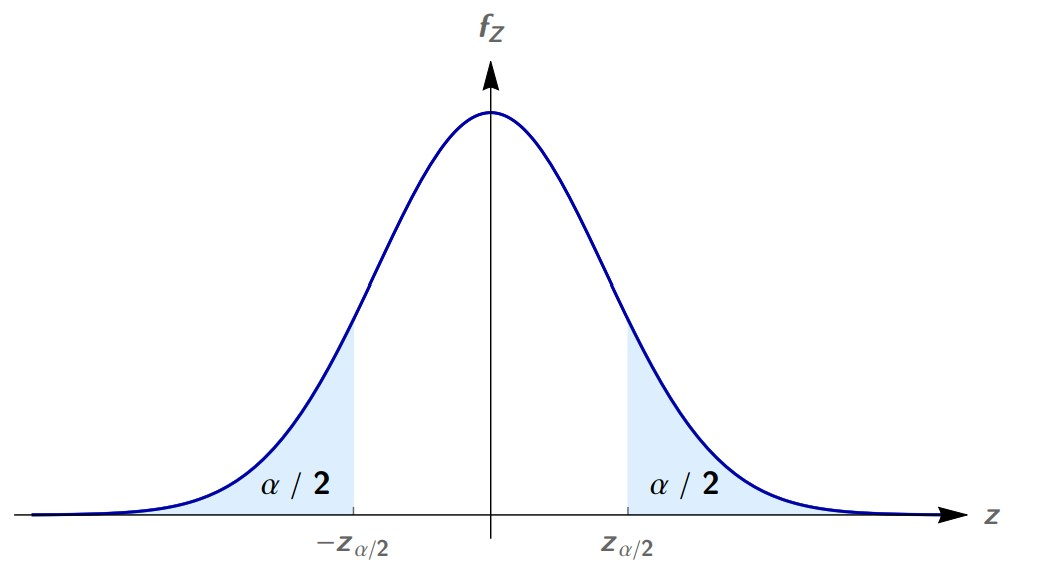
\includegraphics[width=0.37\textwidth,height=0.17\textwidth]{z_value.jpg}
        \caption{Interpretation of z-value}
    \end{figure}\par
    

\end{frame}

\begin{frame}
    \frametitle{$\sigma^2$ doesn't know}
    Three important conclusions:
    \begin{enumerate}
        \item $\overline{X}$ and $S^2$ are independent
        \item $\overline{X}\sim N(\mu, \frac{\sigma^2}{n})$
        \item $\frac{(n-1)S^2}{\sigma^2}\sim \chi^2_{n-1}$
    \end{enumerate}
    

\end{frame}

\begin{frame}
    \frametitle{Confidence interval for $\sigma^2$}

    The two-side confidence interval for $\sigma^2$ is
    \[[\frac{(n-1)S^2}{\chi_{\alpha/2,n-1}^2},\frac{(n-1)S^2}{\chi_{1-\alpha/2,n-1}^2}]\]
    A $100(1-\alpha)\%$ upper confidence interval for $\sigma^2$ is given by
    \[[0,\frac{(n-1)S^2}{\chi_{1-\alpha,n-1}^2}]\]
    A $100(1-\alpha)\%$ lower confidence interval for $\sigma^2$ is given by
    \[[\frac{(n-1)S^2}{\chi_{\alpha,n-1}^2},+\infty)\]

\end{frame}
\begin{frame}
    \frametitle{Confidence interval for $\mu$ ($\sigma^2$ unknown)}
    A student T distribution with freedom $\gamma$ is defined as
    \[T_{\gamma}:=\frac{Z}{\sqrt{\chi^2_{\gamma}/\gamma}}\]
    And we have
    \[\frac{\overline{X}-\mu}{S/\sqrt{n}}=T_{n-1}\]
    With $\sigma$ unknown, a $100(1-\alpha)\%$ two-sided confidence interval on $\mu$ is given by\[
    \overline{X}\pm\frac{t_{\alpha/2,n-1}\cdot S}{\sqrt{n}}\]

\end{frame}

\begin{frame}
    \frametitle{ex 4}

    (See the midterm exam in 22SP)

\end{frame}

\section{Q\&A}
\begin{frame}
    \frametitle{Outline}
    \tableofcontents[currentsection]
\end{frame}
\begin{frame}
    \frametitle{Q\&A}
    Good luck for your midterm exam. \par
    \vspace{0.3cm}
    But if you rely on the luck, not the solid basis of probability theory, you may be in trouble.
    

\end{frame}

\end{document} 